\documentclass[a4paper,11pt,oneside,openany]{jsarticle}
\usepackage[dvipdfmx]{graphicx}
\usepackage{amsmath,amssymb}
\usepackage{bm}
\usepackage{graphicx}
\usepackage{ascmac}

\thispagestyle{empty}
%
\begin{document}
\begin{center}

  \vspace*{35mm}
  \huge 計算機科学実験及演習3 \par
  機能設計仕様書\\
  \vspace{90mm}
  \Large 提出期限:2019/6/14\\
   提出日: \today \\
  \vspace{15mm}
  \Large グループ番号: 9    \\
   1029293806\hspace{5mm}大山 偉永\par

  \vspace{10mm}
\end{center}
\clearpage
\addtocounter{page}{-1}

\newpage

\section{設計を担当したコンポーネントの機能設計仕様(中間報告からの追加分)}
\subsection{即値加算命令ADDI}
即値加算命令実行のためには既存のコンポーネントに変更を与えた。LD命令と同様にADDI命令の時はsign\_ext(d)とr[Rb]の値を足す必要があるのでロードの時に用いたマルチプレクサ(ロードの時はレジスタから来たr[Ra]の値ではなく符号拡張した値sign\_ext(d)を出力するマルチプレクサ)を流用しaddiの時にもこれの制御線を1に設定するように変更する。そうすることでaddiのときにも即値とr[Rb]の和を計算することができるようになる。

\subsection{ジャンプ命令JMP}
ジャンプ命令実行のためにいくつかのコンポーネントを追加した。図\ref{jump}のように、PCに1足した値と分岐命令による符号拡張したアドレスが入力のマルチプレクサの出力を入力の一つとし、もう一方は符号拡張した値sign\_ext(d)を入力としたjumpという制御線を持つマルチプレクサをPCの前段に置く。こうすることでジャンプ命令の時は符号拡張した値がそのままアドレスとしてPCに入力される。

\begin{figure}[h]
  \centering
  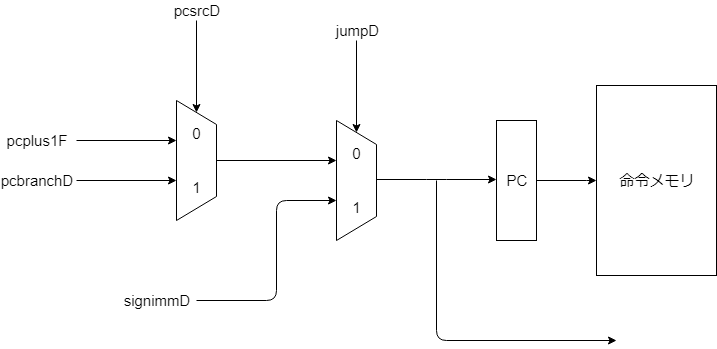
\includegraphics[width=10cm]{jump.png}
  \caption{プログラムカウンタ周辺の回路図}
  \label{jump}
\end{figure}

\section{設計を担当したコンポーネント単体の性能評価}
自分はマルチプレクサからALU等の細かい部品を作成し、フォワーディングユニッ ト、ハザード検出、制御部、全てのコンポーネントを繋ぐ作業はペアの分担である。このレポートでは自分の担当の中で主要なものであるALUの性能評価を記述する。
\subsection{ALU}
\begin{description}
  \item[LE数] 389
  \item[クリティカルパス] 入力aからZフラグの出力までで遅延時間22.3ns
\end{description}}

\section{考察・感想}
中間デモからはハードはペアが大目に担当し僕がソートコンテスト用のアルゴリズムの作成とアセンブラの作成を担当した。ハードのデバッグは比較的やりやすかったものの、ソートのアセンブリのデバッグは本当に困難だった。コンパイルエラーのようなデバッグの手がかりが一切ないためシュミレーションで一つずつプログラムカウンタと命令列を見比べてその内容が正しいか確認する作業は本当に骨の折れる作業だった。またソートコンテストについてrandom.mifをソートしたときのサイクル数は自分たちの一つ上の順位の班のサイクル数より自分たちの班のほうが少なく実装できていたのに、昇順済みデータと降順ソート済みデータについては大きくサイクル数を離されていた。あとから昇順済みデータ降順ソート済みデータについてなぜそんなにサイクル数を小さくすることができたのか本人たちに聞いたところ、初めに昇順データ、降順ソート済みデータで場合分けするようにしていたと聞いてとても悔しかった。今回のソートコンテスト専用にチューニングしたアルゴリズムに負けたということである。現にrandomをソートする場合は自分たちの班のCPUのほうがサイクル数は少なく済んでいたのでとても悔しかった。ハード面ではそもそもそこまで自分たちの班のものは優れていないので高い順位を目指すことはできなかったが、ほかの班と同様にソートコンテスト専用に対応したアルゴリズムで挑戦していたおそらく1msはきれたと思われる。(結果は6位で1.8msだった)せめてほかの人たちがそのようなずるともいえるアルゴリズムでしていることを先に知っていればもう少し改善できたのにととても悔やまれる。
自分たちの班はfmax値が74Mhzで実験を終えたがこれでもタイミング制約をぎりぎりまで詰めた結果であり最高周波数が170Mhzとかの班は本当にどうやったらそんな値になるのか知りたい限りである。そもそも自分たちの班の全体のクリティカルパスはWBステージからレジスタに書き込むまでの部分であり、そのWBステージの値のレジスタ書き込みのタイミングもPLLを用いてクロックの周期を202.5度ずらしたものを使用したが(このタイミングでのレジスタ書き込みが一番クリティカルパスとしての遅延時間を減らすことができた)これ以上の改善はどうしようもなかった。なぜならレジスタへの書き込みはどうしても同じフェーズで行うしかないからである。ゆえに170MHzのような値を出している班は本当にどのようになっているのか不思議である。\\
このcpu実験(特にソートコンテストで)でハード面ではないもののアルゴリズムのすごさが再確認された。また計算量も今まで深く意識したことがなかったがこれを機にコーディングで計算量を意識するきっかけとなった。もちろんハード面でも今回は静的分岐予測を実装したCPUだったのでそのようなハードの制約も意識したコーディングも身につくきっかけになったと思う。\\
もう少し時間があれば投機実行などさらなる改善を施したかったが時間の制約上これ以上は厳しかった。また自分はペアに恵まれたものの本当にペアに依存する実験で友人はやる気のない人と組まされておりもう少し別の実験のやり方があるように思える。グループの人数を東大のように増やすなど。
\end{document}
